\documentclass{ximera}

\input{../../../preamble.tex}


\definecolor{fvdnavy}{HTML}{071D43}
\definecolor{fvdcyan}{HTML}{20BFC6}
\definecolor{fvdcyanlight}{HTML}{EFFCFB}
\definecolor{fvdmagenta}{HTML}{F10D69}
\definecolor{fvdmagentalight}{HTML}{FFF1F7}
\definecolor{fvdtext}{HTML}{163044}





%=================================================
% Pedagogische omgevingen
% PDF: tcolorbox
% HTML: learning-box
%=================================================

\newenvironment{voorkennis}
{%
    \ifdefined\HCode
        \HCode{%
<section class="learning-box learning-box--prior">
<div class="learning-box__header">
<span class="learning-box__icon" aria-hidden="true"></span>
<span class="learning-box__title">Voorkennis</span>
</div>
<div class="learning-box__content">
        }%
        \begin{itemize}
    \else
       \begin{tcolorbox}[
    enhanced,
    breakable,
    colback=fvdcyanlight,
    colframe=fvdcyan,
    coltext=fvdtext,
    boxrule=0.5pt,
    leftrule=4pt,
    arc=4mm,
    outer arc=4mm,
    left=7mm,
    right=6mm,
    top=5mm,
    bottom=5mm,
    before skip=6mm,
    after skip=6mm,
    title=Voorkennis,
    coltitle=fvdcyan,
    fonttitle=\bfseries\Large,
    attach title to upper={\par\smallskip},
    boxed title style={
        empty,
        left=0mm,
        right=0mm,
        top=0mm,
        bottom=0mm
    },
    overlay={
        \draw[
            fvdcyan,
            line width=0.5pt
        ]
        ([xshift=42mm,yshift=-13mm]frame.north west)
        --
        ([xshift=-7mm,yshift=-13mm]frame.north east);
    }
]
        \begin{itemize}
    \fi
}
{%
    \end{itemize}
    \ifdefined\HCode
        \HCode{%
</div>
</section>
        }%
    \else
        \end{tcolorbox}
    \fi
}


\newenvironment{leerdoelen}
{%
    \ifdefined\HCode
        \HCode{%
<section class="learning-box learning-box--goals">
<div class="learning-box__header">
<span class="learning-box__icon" aria-hidden="true"></span>
<span class="learning-box__title">Leerdoelen</span>
</div>
<div class="learning-box__content">
        }%
        \begin{itemize}
    \else
\begin{tcolorbox}[
    enhanced,
    breakable,
    colback=fvdmagentalight,
    colframe=fvdmagenta,
    coltext=fvdtext,
    boxrule=0.5pt,
    leftrule=4pt,
    arc=4mm,
    outer arc=4mm,
    left=7mm,
    right=6mm,
    top=5mm,
    bottom=5mm,
    before skip=6mm,
    after skip=6mm,
    title=Leerdoelen,
    coltitle=fvdmagenta,
    fonttitle=\bfseries\Large,
    attach title to upper={\par\smallskip},
    boxed title style={
        empty,
        left=0mm,
        right=0mm,
        top=0mm,
        bottom=0mm
    },
    overlay={
        \draw[
            fvdmagenta,
            line width=0.5pt
        ]
        ([xshift=42mm,yshift=-13mm]frame.north west)
        --
        ([xshift=-7mm,yshift=-13mm]frame.north east);
    }
]
        \begin{itemize}
    \fi
}
{%
    \end{itemize}
    \ifdefined\HCode
        \HCode{%
</div>
</section>
        }%
    \else
        \end{tcolorbox}
    \fi
}



\title{Nulwaarden en tekenverloop}
\author{Ingmar Herreman}

\begin{document}

% FVD_CHAPTER_DATA_START
% Automatisch gegenereerd uit index.tex.
% Niet handmatig aanpassen.
\fvdchapterdata{5}{Het gedrag van functies beschrijven}{1}
% FVD_CHAPTER_DATA_END



\begin{abstract}
Een grafiek vertelt waar een functie nul, positief of negatief is.
In dit hoofdstuk leren we die informatie grafisch en algebraïsch
onderzoeken en samenvatten in een tekentabel.
\end{abstract}

\maketitle

\begin{voorkennis}

    \item Je kunt een functievoorschrift interpreteren en gebruiken om functiewaarden te bepalen.
  
    \item Je kunt het domein van een functie bepalen en beelden en originelen vinden.
  
    \item Je kunt vergelijkingen algebraïsch oplossen.
  
    \item Je kunt eenvoudige veeltermen ontbinden in factoren.
  
    \item Je kunt een grafiek lezen en punten op de grafiek verbinden met hun coördinaten.
  
  \end{voorkennis}
  
  \begin{leerdoelen}
  
    \item Je kunt het onderscheid uitleggen tussen een nulwaarde van een functie en het bijbehorende nulpunt van de grafiek.
  
    \item Je kunt nulwaarden uit een grafiek aflezen en ze, wanneer het functievoorschrift dit toelaat, algebraïsch bepalen.
  
    \item Je kunt uit een grafiek bepalen op welke intervallen \(f(x)>0\), \(f(x)=0\) en \(f(x)<0\).
  
    \item Je kunt het tekenverloop van een functie onderzoeken en de resultaten overzichtelijk weergeven in een tekentabel.
  
    \item Je kunt bij het onderzoeken van het tekenverloop rekening houden met waarden die niet tot het domein van de functie behoren.
  
    \item Je kunt de informatie over nulwaarden en tekenverloop met elkaar verbinden in een grafiek, een functievoorschrift en een tekentabel.
  
    \item Je kunt aan de hand van het gedrag van de grafiek verklaren waarom een nulwaarde niet noodzakelijk een tekenwisseling veroorzaakt.
  
    \item Je kunt de betekenis van nulwaarden en het teken van een functie interpreteren binnen een concrete context en je conclusies terugkoppelen naar de oorspronkelijke situatie.
  
  \end{leerdoelen}


% ============================================================
% 1. EEN GRAFIEK VERTELT MEER DAN WAARDEN
% ============================================================

\FVDsection{Boven, op of onder de \(x\)-as}

Een grafiek geeft niet alleen afzonderlijke functiewaarden weer.
Aan haar ligging ten opzichte van de \(x\)-as zien we onmiddellijk
welk teken de functiewaarden hebben.

\[
\begin{array}{ccl}
\text{grafiek boven de \(x\)-as}
&\Longleftrightarrow& f(x)>0,\\[2mm]
\text{grafiek op de \(x\)-as}
&\Longleftrightarrow& f(x)=0,\\[2mm]
\text{grafiek onder de \(x\)-as}
&\Longleftrightarrow& f(x)<0.
\end{array}
\]

\begin{center}
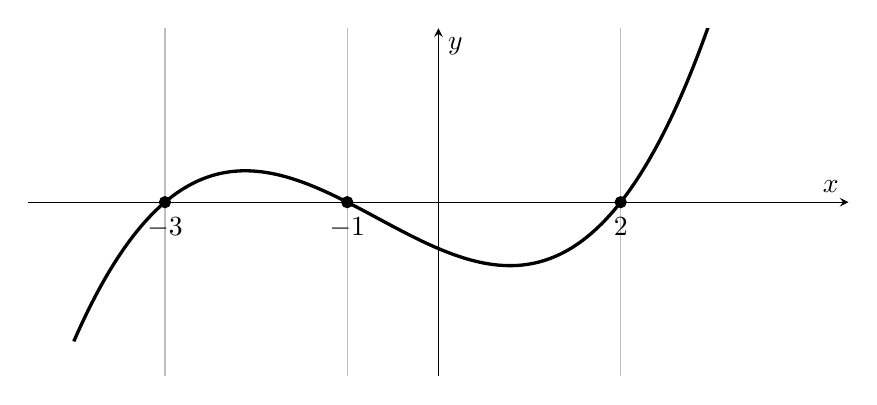
\begin{tikzpicture}
\begin{axis}[
    width=12cm,
    height=6cm,
    axis lines=middle,
    xmin=-4.5,xmax=4.5,
    ymin=-4.5,ymax=4.5,
    xlabel={$x$},ylabel={$y$},
    grid=both,
    samples=200,
    xtick={-3,-1,2},
    ytick=\empty
]
\addplot[very thick,domain=-4:4] {(x+3)*(x+1)*(x-2)/5};
\addplot[only marks,mark=*,mark size=2pt]
coordinates {(-3,0) (-1,0) (2,0)};
\end{axis}
\end{tikzpicture}
\end{center}

In deze grafiek zijn \(x=-3\), \(x=-1\) en \(x=2\)
bijzondere waarden: daar ligt de grafiek op de \(x\)-as.
Die waarden verdelen het domein in intervallen waarop de functie
positief of negatief is.

Dat verband tussen de ligging van de grafiek en het teken van
de functiewaarden staat centraal in dit hoofdstuk.


% ============================================================
% 2. NULWAARDEN EN NULPUNTEN
% ============================================================

\FVDsection{Nulwaarden en nulpunten}

\begin{definitie}
Een getal \(a\) is een \textbf{nulwaarde} van een functie \(f\) als

\[
f(a)=0.
\]

Het bijbehorende punt

\[
(a,0)
\]

op de grafiek noemen we een \textbf{nulpunt}.
\end{definitie}

Een nulwaarde is dus een \emph{\(x\)-waarde};
een nulpunt is een \emph{punt van de grafiek}.

Grafisch zoeken we de nulwaarden waar de grafiek de \(x\)-as
\textbf{snijdt of raakt}.

Algebraïsch lossen we de vergelijking

\[
f(x)=0
\]

op.

\begin{voorbeeld}[Grafisch en algebraïsch]

Neem

\[
f(x)=x^2-x-6.
\]

Om de nulwaarden algebraïsch te bepalen, lossen we op:

\[
x^2-x-6=0.
\]

Ontbinden geeft

\[
(x-3)(x+2)=0,
\]

dus

\[
x=-2
\qquad\text{of}\qquad
x=3.
\]

De nulwaarden zijn \(-2\) en \(3\).
De nulpunten zijn

\[
(-2,0)
\qquad\text{en}\qquad
(3,0).
\]

\begin{center}
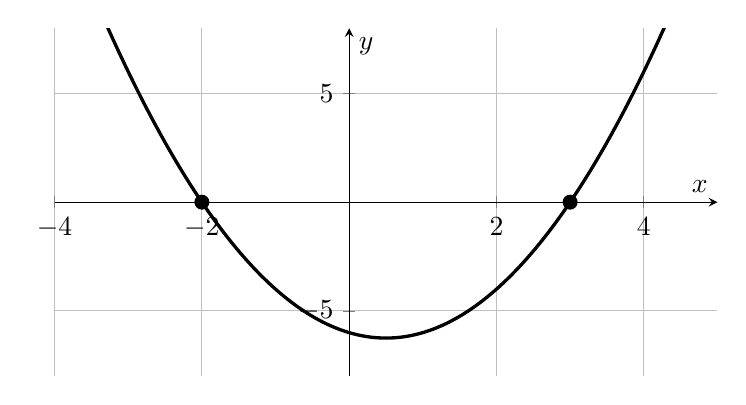
\begin{tikzpicture}
\begin{axis}[
    width=10cm,height=6cm,
    axis lines=middle,
    xmin=-4,xmax=5,
    ymin=-8,ymax=8,
    xlabel={$x$},ylabel={$y$},
    grid=both,
    samples=200
]
\addplot[very thick,domain=-3.5:4.5] {x^2-x-6};
\addplot[only marks,mark=*,mark size=2.5pt]
coordinates {(-2,0) (3,0)};
\end{axis}
\end{tikzpicture}
\end{center}

De grafische en algebraïsche informatie vertellen hetzelfde verhaal.
\end{voorbeeld}


% ============================================================
% 3. EEN NULWAARDE IS NIET ALTIJD EEN TEKENWISSEL
% ============================================================

\FVDsection{Snijden of raken?}

Het is verleidelijk om te denken dat een functie bij elke nulwaarde
van teken verandert. Dat is niet zo.

Vergelijk

\[
f(x)=x-2
\qquad\text{en}\qquad
g(x)=(x-2)^2.
\]

Beide functies hebben \(x=2\) als nulwaarde.

\begin{center}
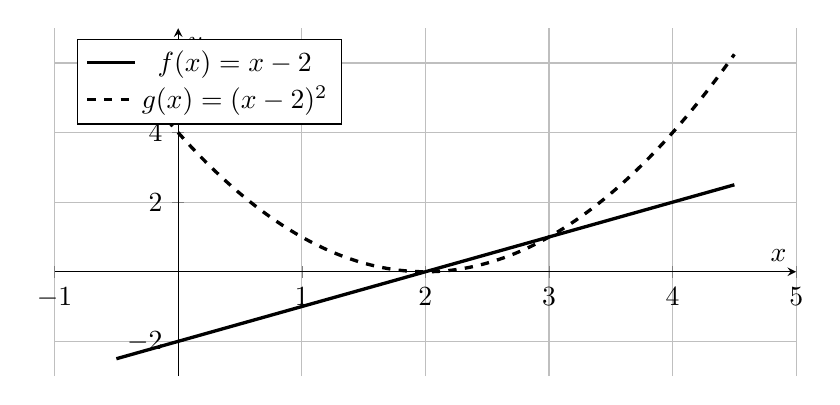
\begin{tikzpicture}
\begin{axis}[
    width=11cm,height=6cm,
    axis lines=middle,
    xmin=-1,xmax=5,
    ymin=-3,ymax=7,
    xlabel={$x$},ylabel={$y$},
    grid=both,
    samples=200,
    legend style={at={(0.03,0.97)},anchor=north west}
]
\addplot[very thick,domain=-0.5:4.5] {x-2};
\addlegendentry{\(f(x)=x-2\)}
\addplot[very thick,dashed,domain=-0.5:4.5] {(x-2)^2};
\addlegendentry{\(g(x)=(x-2)^2\)}
\end{axis}
\end{tikzpicture}
\end{center}

Voor \(f\) gaat de grafiek door de \(x\)-as:

\[
x<2 \Rightarrow f(x)<0,
\qquad
x>2 \Rightarrow f(x)>0.
\]

Er is dus een \textbf{tekenwisseling}.

Voor \(g\) raakt de grafiek de \(x\)-as, maar blijft ze aan beide
zijden erboven:

\[
g(x)\geq 0.
\]

Er is bij \(x=2\) dus \textbf{geen tekenwisseling}.

\begin{opmerking}[Kijk naar het gedrag, niet alleen naar de nulwaarde]
Uit \(f(a)=0\) volgt alleen dat de grafiek door het punt \((a,0)\) gaat.
Of het teken verandert, moet je uit de grafiek, het voorschrift
of een tekenonderzoek afleiden.
\end{opmerking}


% ============================================================
% 4. TEKENVERLOOP
% ============================================================

\FVDsection{Het tekenverloop van een functie}

\begin{definitie}
Het \textbf{tekenverloop} van een functie beschrijft voor welke
waarden van \(x\)

\[
f(x)>0,\qquad f(x)=0,\qquad f(x)<0.
\]

Een \textbf{tekentabel} vat die informatie overzichtelijk samen.
\end{definitie}

Voor

\[
f(x)=x^2-x-6=(x+2)(x-3)
\]

zijn de nulwaarden \(-2\) en \(3\).
Ze verdelen de reële as in drie intervallen:

\[
]-\infty,-2[,\qquad ]-2,3[,\qquad ]3,+\infty[.
\]

We onderzoeken het teken op elk interval.

\[
\begin{array}{c|ccccc}
x & ]-\infty,-2[ & -2 & ]-2,3[ & 3 & ]3,+\infty[\\
\hline
f(x) & + & 0 & - & 0 & +
\end{array}
\]

Daaruit lezen we bijvoorbeeld:

\[
f(x)<0
\quad\Longleftrightarrow\quad
x\in]-2,3[.
\]

\begin{voorbeeld}[Van voorschrift naar tekentabel]

Onderzoek het teken van

\[
h(x)=(x+1)(x-4).
\]

De nulwaarden zijn

\[
x=-1
\qquad\text{en}\qquad
x=4.
\]

We kunnen per factor redeneren:

\[
\begin{array}{c|ccccc}
x & ]-\infty,-1[ & -1 & ]-1,4[ & 4 & ]4,+\infty[\\
\hline
x+1 & - & 0 & + & + & +\\
x-4 & - & - & - & 0 & +\\
\hline
h(x) & + & 0 & - & 0 & +
\end{array}
\]

Het product is positief wanneer de factoren hetzelfde teken hebben
en negatief wanneer hun tekens verschillend zijn.
\end{voorbeeld}


% ============================================================
% 5. DOMEINONDERBREKINGEN
% ============================================================

\FVDsection{Niet elke grenswaarde is een nulwaarde}

Bij een tekenonderzoek moeten we niet alleen nulwaarden bekijken.
Ook waarden die \textbf{niet tot het domein behoren} kunnen de reële as
in verschillende intervallen verdelen.

Beschouw

\[
f(x)=\frac{x-1}{x+2}.
\]

De teller is nul voor \(x=1\), dus \(1\) is een nulwaarde.

Voor \(x=-2\) is de noemer nul. De functie is daar niet gedefinieerd:

\[
\operatorname{dom}f=\mathbb{R}\setminus\{-2\}.
\]

De waarden \(-2\) en \(1\) verdelen de reële as in drie intervallen.

\[
\begin{array}{c|ccccc}
x & ]-\infty,-2[ & -2 & ]-2,1[ & 1 & ]1,+\infty[\\
\hline
x-1 & - & - & - & 0 & +\\
x+2 & - & 0 & + & + & +\\
\hline
f(x) & + & \text{n.g.} & - & 0 & +
\end{array}
\]

Hier betekent \(\text{n.g.}\): \emph{niet gedefinieerd}.

\begin{opmerking}
Een waarde die niet tot het domein behoort, is \textbf{geen nulwaarde}.
Toch moet ze in een tekenonderzoek zichtbaar zijn, omdat ze het domein
in afzonderlijke intervallen kan verdelen.
\end{opmerking}


% ============================================================
% 6. EEN BETROUWBARE WERKWIJZE
% ============================================================

\FVDsection{Van voorschrift naar tekenverloop}

Voor een functie waarvan je het teken algebraïsch kunt onderzoeken,
is de volgende werkwijze betrouwbaar.

\begin{eigenschap}[Stappenplan tekenonderzoek]
\begin{enumerate}
    \item Bepaal of controleer het \textbf{domein}.
    \item Bepaal de \textbf{nulwaarden} door \(f(x)=0\) op te lossen.
    \item Noteer ook de waarden waar de functie \textbf{niet gedefinieerd} is.
    \item Verdeel het domein in intervallen met behulp van die bijzondere waarden.
    \item Bepaal op elk interval het teken van \(f(x)\).
    \item Vat het resultaat samen in een \textbf{tekentabel}.
    \item Controleer of de tekentabel overeenkomt met de grafiek.
\end{enumerate}
\end{eigenschap}

Die laatste stap is belangrijk.
Een grafiek is geen vervanging voor een redenering,
maar ze is wel een krachtig middel om een resultaat te controleren.


% ============================================================
% 7. VAN TEKENTABEL TERUG NAAR GRAFIEK
% ============================================================

\FVDsection{Redeneren in de andere richting}

Een tekentabel bevat genoeg informatie om bepaalde kenmerken van
een mogelijke grafiek te voorspellen.

Stel dat

\[
\begin{array}{c|ccccc}
x & ]-\infty,-1[ & -1 & ]-1,3[ & 3 & ]3,+\infty[\\
\hline
f(x) & - & 0 & + & 0 & -
\end{array}
\]

gegeven is.

Dan weten we zonder het voorschrift te kennen:

\begin{itemize}
    \item de grafiek heeft nulpunten \((-1,0)\) en \((3,0)\);
    \item links van \(-1\) ligt ze onder de \(x\)-as;
    \item tussen \(-1\) en \(3\) ligt ze boven de \(x\)-as;
    \item rechts van \(3\) ligt ze opnieuw onder de \(x\)-as;
    \item bij beide nulwaarden vindt een tekenwisseling plaats.
\end{itemize}

\begin{opmerking}[Wat weten we nog niet?]
Een tekentabel bepaalt de grafiek niet volledig.
We weten bijvoorbeeld nog niet waar de functie stijgt of daalt,
waar extrema liggen of hoe snel de functie verandert.
Die eigenschappen onderzoeken we in de volgende hoofdstukken.
\end{opmerking}


% ============================================================
% 8. IN CONTEXT
% ============================================================

\FVDsection{Wat betekent het teken in een context?}

Het teken van een functie krijgt pas betekenis wanneer we weten
wat de functie voorstelt.

\begin{voorbeeld}[Temperatuurverschil]

Het temperatuurverschil tussen een proefopstelling en de omgeving
wordt gemodelleerd door

\[
D(t)=T_{\text{proef}}(t)-T_{\text{omgeving}}(t).
\]

Dan betekent

\[
D(t)>0
\]

dat de proefopstelling warmer is dan de omgeving,

\[
D(t)<0
\]

dat ze kouder is, en

\[
D(t)=0
\]

dat beide temperaturen gelijk zijn.

Een nulwaarde van \(D\) is hier dus niet zomaar een snijpunt met
de \(t\)-as: ze stelt een fysisch betekenisvol tijdstip voor.
\end{voorbeeld}

\begin{opmerking}[Demathematiseren]
Schrijf in een context niet alleen
``\(D(t)<0\)''.
Vertaal het resultaat terug naar de werkelijkheid:
``de proefopstelling is op dat tijdstip kouder dan de omgeving''.
\end{opmerking}


% ============================================================
% 9. GEOGEBRA
% ============================================================

\FVDsection{Onderzoeken met GeoGebra}

Gebruik GeoGebra om het verband tussen grafiek, nulwaarden
en tekenverloop te onderzoeken.

Voer bijvoorbeeld in:

\[
f(x)=(x+2)(x-1)^2(x-4).
\]

Onderzoek eerst de grafiek zonder een tekentabel te maken.

\begin{enumerate}
    \item Zoek de nulwaarden.
    \item Voorspel bij welke nulwaarden het teken verandert.
    \item Bepaal grafisch waar \(f(x)>0\) en waar \(f(x)<0\).
    \item Stel daarna algebraïsch de tekentabel op.
    \item Vergelijk beide resultaten.
    \item Verander de factor \((x-1)^2\) in \((x-1)\). Wat verandert er?
\end{enumerate}

\begin{opmerking}
GeoGebra wordt hier gebruikt om een vermoeden te vormen en een
redenering te controleren. De grafiek alleen is niet het eindantwoord.
\end{opmerking}


% ============================================================
% 10. SAMENVATTING
% ============================================================

\FVDsection{Samenvatting}

\[
\boxed{
\text{grafiek}
\longleftrightarrow
\text{nulwaarden}
\longleftrightarrow
\text{tekenverloop}
\longleftrightarrow
\text{tekentabel}
\longleftrightarrow
\text{voorschrift}
}
\]

Onthoud vooral:

\begin{itemize}
    \item \(a\) is een nulwaarde als \(f(a)=0\);
    \item \((a,0)\) is het bijbehorende nulpunt;
    \item boven de \(x\)-as is \(f(x)>0\), onder de \(x\)-as is \(f(x)<0\);
    \item een nulwaarde veroorzaakt niet noodzakelijk een tekenwisseling;
    \item domeinonderbrekingen moeten in een tekenonderzoek worden opgenomen;
    \item een tekentabel en een grafiek beschrijven hetzelfde tekenverloop
          in verschillende voorstellingen;
    \item in toepassingen moet het teken opnieuw in de context worden geïnterpreteerd.
\end{itemize}

\end{document}
